\documentclass[]{article}
% used packages
\usepackage[german]{babel}   % enables umlaute
\usepackage[utf8]{inputenc}  % set encoding to utf8 otherwise no umlaute
\usepackage{graphicx}        % for including graphics
\usepackage{hyperref}        % for using hyperlinks in the document
\usepackage{tabularx}        % for extending tabluar
\usepackage{multirow}        % for rowspan in tabularx
\usepackage{ltablex}         % tables over multiple pages
\usepackage{textcmds}        % for quote support
\usepackage{pdfpages}        % for pdf include
\usepackage{caption}
\usepackage{minted}
\usepackage{listings}
\usepackage[left=1.0in, right=1.0in, top=1.0in, bottom=1.0in]{geometry} % for custom page layout

% Title Page
\title{Raspberry PI Security Application}
\author{Thonas Herzog, Philipp Wurm}


\newcommand{\imageDir}{images}
\newcommand{\dockerTestDir}{../java/testsuite/client/src/main/resources/docker}
\newcommand{\dockerRPIDir}{../host/docker}
\renewcommand\listingscaption{Quelltext}

\newenvironment{code}{\captionsetup{type=listing}}{}

\newmintedfile[yamlFile]{yaml}{
	linenos=true, 
	frame=single, 
	breaklines=true, 
	tabsize=2,
	numbersep=5pt,
	xleftmargin=10pt,
	baselinestretch=1,
	fontsize=\footnotesize
}

\begin{document}
\maketitle

\begin{abstract}
\end{abstract}

\section{Einleitung}
Diese Dokument stellt die Dokumentation des Projekts \emph{Raspberry PI Security Application}, in weiterer Folge \emph{RPISec} genannt, dar, das für die Lehrveranstaltung \emph{Mobile und ubiquitäre Systeme} realisiert wurde. In diesem Projekt wurde eine Heimsicherheitsanwendung mit Raspberry PI, Docker und Spring realisiert, die bei einem Sicherheitsverstoß in der Lage ist, bekannte mobile Endgeräte von registrierten Benutzern über diesen Sicherheitsverstoß zu informieren. 

\section{Problemdarstellung}
Dieser Abschnitt behandelt die Problemdarstellung, welche die Grundlage für die zu implementierende \emph{Raspberry PI Security Application} ist. Bei einem Auslösen eines Bewegungssensors in einem Haushalt sollen alle Bewohner über ihre mobilen Endgeräte wie Handy und Tablet über den Vorfall informiert werden sowie ein Foto erhalten, das den Sicherheitsbereich, zum Zeitpunkt wann der Bewegungsmelder ausgelöst wurde, zeigt. Des weiteren soll es zu jedem Zeitpunkt möglich sein sich ein aktuelles Foto des Sicherheitsbereichs über ein mobiles Endgerät zu beziehen.  
\newline
\newline
Da es sich um eine Sicherheitsanwendung handelt, soll die Benutzerverwaltung sowie die Authentifizierung \emph{In-House} gehalten werden, also die Sicherheitsanwendung selbst soll in der Lage sein die Benutzer zu verwalten und die Authentifizierungen durchzuführen. Da sich die mobilen Endgeräte in irgendwelchen Netzen ans Internet anbinden können, wie zum Beispiel über einen Mobilfunkanbieter, Internetanbieter oder öffentlichen \emph{Hot-Spot}, wird ein \emph{Messaging} Dienst benötigt über den die mobilen Endgeräte erreicht werden können. Dieser muss es erlauben, dass die Benutzerverwaltung von einem anderen Dienst übernommen werden kann, da wir diesen \emph{Messaging} Dienst nicht vertrauen wollen und daher den \emph{Messaging} Dienst auch nicht die Benutzerverwaltung überlassen wollen.
\newpage

\section{Funktionsweise}
Dieser Abschnitt behandelt die Funktionsweise der Applikation \emph{RPISec}. Die Abbildung \ref{fig:image-system-structure} zeigt den Systemaufbau der \emph{RPISec} Applikation. 
\begin{figure}[h]
	\centering
	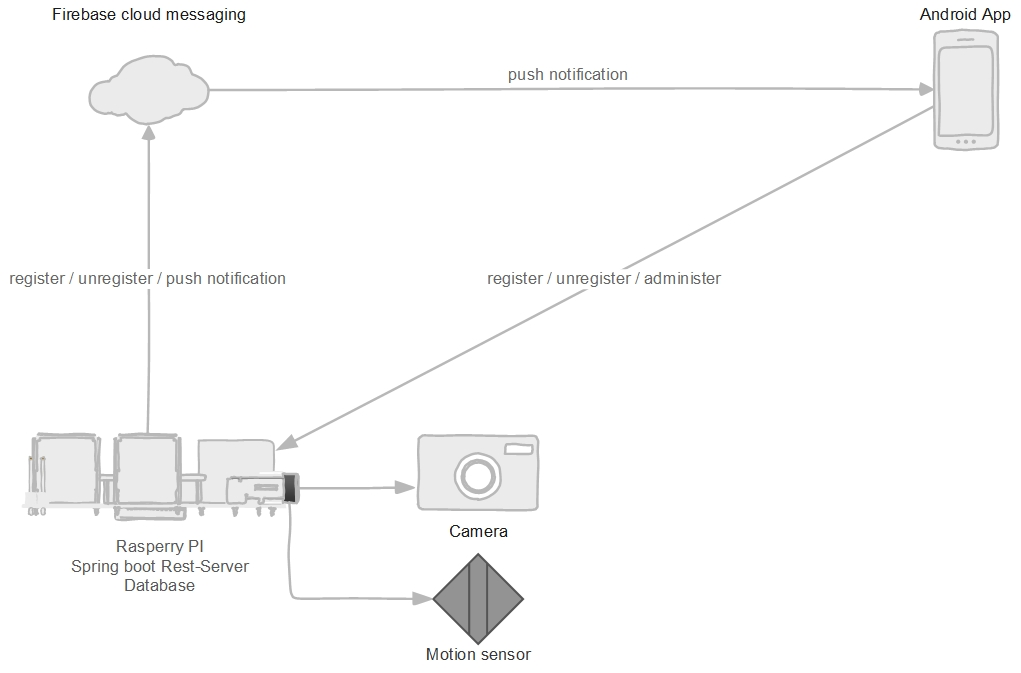
\includegraphics[scale=0.6]{\imageDir/Infrastructure.jpg}
	\caption{Systemaufbau der \emph{RPISec} Applikation}
	\label{fig:image-system-structure}
\end{figure}
\begin{figure}[h]
	\centering
	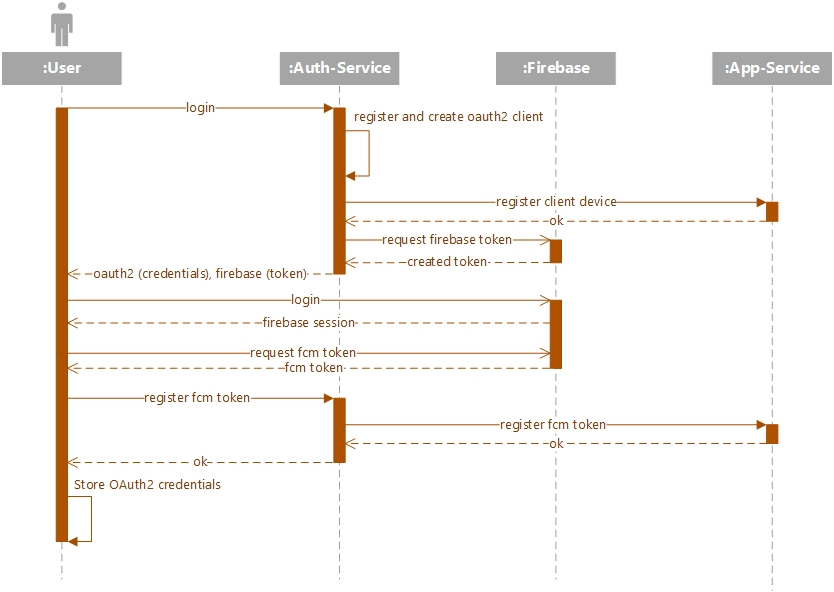
\includegraphics[scale=0.55]{\imageDir/sequence-client-login.jpg}
	\caption{Sequenzdiagramm des Logins über einen mobilen \emph{Client}}
	\label{fig:image-sequence-client-login}
\end{figure}
\ \newline
Die folgende Abbildung \ref{fig:image-sequence-client-login} zeigt das Sequenzdiagramm das den erfolgreichen Ablauf des Logins eines Benutzers über ein Android Gerät beschreibt. Im Zuge des Logins wird das mobile Endgerät am Authentifizierungsservice und Applikationsservice registriert und für jeden Login ein neuer \emph{OAuth2 Client} angelegt und gegebenenfalls der alte \emph{OAuth2 Client} für dieses Endgerät gelöscht. Bezüglich OAuth2 wurde dieser Ansatz gewählt, da mit der \emph{Client}-Applikation keine \emph{Oauth2 Client} Zugangsdaten ausgeliefert sollen.
\ \newpage
\begin{figure}[h]
	\centering
	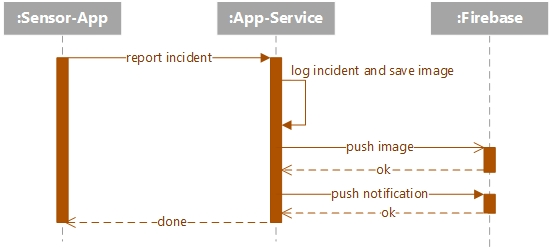
\includegraphics[scale=0.55]{\imageDir/sequence-incident.jpg}
	\caption{Sequenzdiagramm des Behandelns eines Sicherheitsvorfalls}
	\label{fig:image-sequence-incident}
\end{figure}
\ \newline
Die Abbildung \ref{fig:image-sequence-incident} zeigt das Sequenzdiagramm für das Behandeln eines Sicherheitsvorfalls, der von der Sensorapplikation erkannt wurde und dem Applikationsservice mitgeteilt wurde.  
\begin{figure}[h]
	\centering
	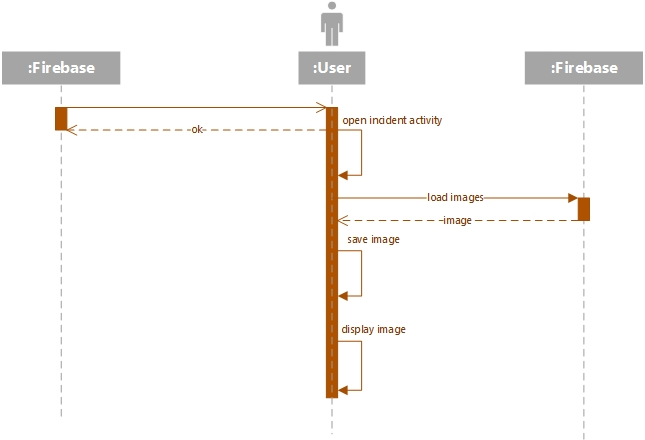
\includegraphics[scale=0.55]{\imageDir/sequence-client-notification.jpg}
	\caption{Sequenzdiagramm der Benachrichtigung eines \emph{Client}}
	\label{fig:image-sequence-client-notification}
\end{figure}
\ \newline
Die Abbildung \ref{fig:image-sequence-client-notification} zeigt den Ablauf einer  Benachrichtigung eines \emph{Client} über den \emph{Firebase Messaging} Dienst. Nachdem auf die Nachricht geklickt wurde, wird eine \emph{Activity} für das Anzeigen der Bilder geöffnet, die alle bereits gespeicherten Bilder und das neu geladene Bild anzeigt. 

\section{Hardware}
Dieser Abschnitt behandelt die verwendete Hardware für \emph{RPISec}. Für den Testaufbau wurden folgende Hardwarekomponenten verwendet.
\begin{itemize}
	\item Ein \emph{Raspberry PI 3 Model B}\footnote{\url{https://www.raspberrypi.org/products/raspberry-pi-3-model-b/}},
	\item \emph{AZDeliveryCamRasp}\footnote{\url{https://az-delivery.de/products/raspberrykamerav1-3}} und ein
	\item \emph{HC-SR501\footnote{\url{https://www.mpja.com/download/31227sc.pdf}} Bewegungssensor}.
\end{itemize}
\ \newpage
\begin{figure}[h]
	\centering
	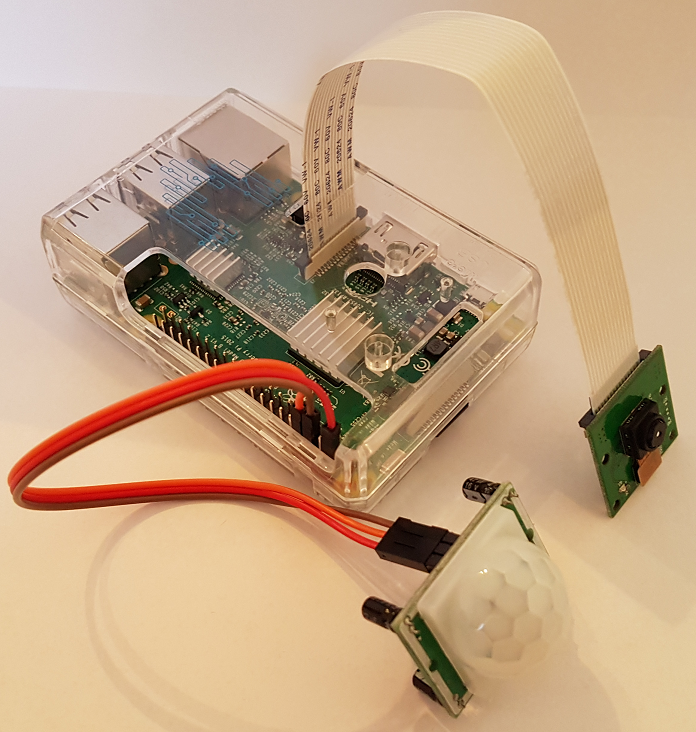
\includegraphics[scale=0.45]{\imageDir/rpisec-hardware-setup.png}
	\caption{Testaufbau der Applikation}
	\label{fig:image-hardware-setup}
\end{figure}
\ \newline
Wie in Abbildung \ref{fig:image-hardware-setup} zu ersichtlich ist, wurde die Kamera über CSI \emph{(Camera-Serial-Interface)}) und der Bewegungssensor über GPIO \emph{(General Purpose Input/Output)} an den \emph{Raspberry PI} angeschlossen.

\section{Betriebssysteme}
Dieser Abschnitt behandelt die verwendete Betriebssysteme für den \emph{Raspberry PI}. Die Applikation \emph{RPISec} wurde einerseits mit dem Betriebssystem \emph{hypriotos-rpi} und andererseits mit \emph{Raspian} realisiert. Das Betriebssystem \emph{hypriots} basiert auf \emph{Debian Jessie} und wird von dem \emph{OpenSource} Projekt \emph{hypriot}\footnote{\url{https://blog.hypriot.com/}} zur Verfügung gestellt wird. Das Ziel von \emph{hypriots} ist es ein Betriebssystem für \emph{Raspberry PI} zur Verfügung stellen, das bereits Docker vorinstalliert und betriebsbereit hat. Mit dem Betriebssystem \emph{Raspian} muss Docker selbst installiert, wobei Docker als Paket im \emph{Repository} zur Verfügung steht und daher sich die Installation als unkompliziert gestaltet.
\newline
\newline
Wenn Docker installiert und betriebsbereit ist, dann spielt es keine Rolle auf welchem Betriebssystem die Applikation \emph{RPISec} betrieben wird.
\newline
\newline
Da die Applikation \emph{RPISec} auf eine aktive Internetverbindung angewiesen ist, muss das Betriebssystem so konfiguriert werden, dass der \emph{Raspberry PI} entweder über \emph{Ethernet} oder \emph{Wlan} an ein Netzwerk angebunden ist, das Zugriff auf das Internet erlaubt. In einem produktiven Betrieb muss der \emph{Raspberry PI} über das Internet erreichbar sein, damit die mobilen \emph{Clients} Anfragen an die gehosteten \emph{Microservice} absetzen können.
\ \newpage

\section{Software}
Dieser Abschnitt behandelt die verwendete bzw. implementierte Software für \emph{RPISec}.
\subsection{Services und \emph{Cloud}}
Dieser Abschnitt behandelt die auf dem \emph{Raspberry PI} gehosteten Services. Die Services wurden mit \emph{Spring Boot} als \emph{Microservices} implementiert, was möglich war, da Oracle eine ARM Implementierung der Java-JDK bereitstellt und die \emph{Microservices} schlank implementiert wurden, sodass die zur Verfügung stehenden Ressourcen ausreichen, um diese Services auf einen \emph{Raspberry PI} zu betreiben.
\newline
\newline
Es wurden die beiden \emph{Microservices} \emph{rpisec-auth-service} für die Benutzerverwaltung und OAuth2 Authentifizierung und \emph{rpisec-app-service} für die Interaktion mit der Sensorik und der Interaktion mit dem \emph{Cloud}-Diensten implementiert, wobei der \emph{Microservice} \emph{rpisec-auth-service} im Zuge des Projekts für die Lehrveranstaltung \emph{Service Engineering} implementiert wurde. Es hätte auch ausgereicht die Benutzerverwaltung in den \emph{Microservice rpisec-app-service} zu verpacken, obwohl dann der \emph{Microservice} für zwei Aspekte verantwortlich gewesen wäre was im Widerspruch zu einem \emph{Microservice} steht, der nur für einen Aspekt verantwortlich sein soll. 
\newline
\newline
Der Microservice \emph{rpisec-app-service} interagiert nicht direkt mit der Sensorik, sondern bindet die Sensorapplikation beschrieben in Abschnitt \ref{sec:sensor-application} ein und ist für dessen Lebenszyklus verantwortlich. Nachdem Start der Sensorapplikation wird ein \emph{Listener} registriert, der auf Statusänderungen des Bewegungssensor reagiert und diesen Sicherheitsvorfall wie in Abbildung \ref{fig:image-sequence-incident} behandelt.
\newline
\newline
Die beiden \emph{Microservices} müssen Daten persistent halten und sind daher auf eine Datenbank angewiesen, wobei im Entwicklungsbetrieb auf einen Entwicklerrechner H2 und im produktiven Betrieb auf einen \emph{Raspberry PI} PostgreSQL verwendet wird. Die Datenbank PostgreSQL konnte verwendet werden, da PostgreSQL die ARM Architektur unterstützt.
\newline
\newline
Als \emph{Cloud} Anbieter wurde \emph{Google} gewählt, welcher die Plattform \emph{Firebase} anbietet, die eine JSON-Datenbank und einen \emph{Cloud Messaging} Dienst anbietet. Für diesen Dienst gibt es eine Java Implementierung das sogenannte \emph{firebase-admin-sdk}, das eine API zum Interagieren mit der JSON-Datenbank und eine API zum Erstellen von Authentifizierungstoken für die \emph{Client}-Authentifizierung bei Firebase zur Verfügung stellt. In der Java Implementierung wird zurzeit keine API für die Interaktion mit dem \emph{Messaging} Dienst zur Verfügung gestellt, was aber kein Problem darstellt, da es sich hierbei um eine einfache Anfrage an eine \emph{REST-API} handelt, die mit Spring \emph{RestTemplate} durchgeführt wird.

\subsection{Docker Infrastruktur}
Dieser Abschnitt behandelt die Docker Infrastruktur, welche die Service und deren Abhängigkeiten hosted und verwaltet. Da der Umgang mit Docker und einer umfangreicheren Infrastruktur mit viel Shell-Skripten verbunden ist, wird das Python basierte Tool Docker-Compose verwendet, das es erlaubt eine Infrastruktur, die aus einer Menge von untereinander abhängigen Services besteht, deklarativ über eine \emph{YAML}-Konfigurationsdatei definiert werden kann. 
\newline
\newline
Der Quelltext \ref{src:test-docker-compose} zeigt den Inhalt der \emph{docker-compose.yml}, welche die Docker Infrastruktur für \emph{RPISec} amd \emph{Raspberry PI} definiert. Die in der Datei vorkommenden Textfragmente im Format \emph{\$\{...\}} stellen Variablen dar, die \emph{Docker Compose} entweder aus einer Datei mit dem Namen \emph{.env}, die auf derselben Ebene wie die \emph{docker-compose.yml} platziert werden muss, oder aus den Umgebungsvariablen des Benutzers, mit dem die Infrastruktur erstellt wird, auflöst. Sollten Variablen nicht auflösbar sein, so wird eine entsprechende Meldung auf die Konsole ausgegeben.
\begin{code}
	\caption{docker-compose.yml für RPISec am \emph{Raspberry PI}}
	\yamlFile{\dockerRPIDir/docker-compose.yml}
	\label{src:test-docker-compose}
\end{code}

\subsection{Sensorapplikation}
\label{sec:sensor-application}

\subsection{Mobiler \emph{Client}}


% Quellen
% AZDeliveryPICam:
% https://www.amazon.de/dp/B01M6UCEM5/ref=pe_386171_51767411_TE_dp_3
% -------------------------------------------------------------------
% HC-SR501
% https://www.amazon.de/dp/B00TI2ZC72/ref=pe_386171_38075861_TE_item
% -------------------------------------------------------------------
% HC-SR501 Schema
% ttp://www.netzmafia.de/skripten/hardware/RasPi/Projekt-PIR/
% -------------------------------------------------------------------

\end{document}          
